\documentclass[a4paper,11pt]{article}

\usepackage[plain]{fullpage}
\usepackage{graphicx}  %This enables the inclusion of pdf graphic files in figures
\usepackage[hidelinks]{hyperref} % Make links in your document click-able NB: must be loaded before the caption-package
\usepackage{caption}
\usepackage{subcaption}
\usepackage{wrapfig}


\title{WPS: A user configuration facility that became a threat}
\author{Antonio M. Franques Garcia \\\\
	\texttt{antoniof@stud.ntnu.no}\\
	TTM4137 Wireless Security Technical Essay}
\date{\today}

\begin{document}
\maketitle

\section{Introduction}
In this essay we will first present the Wi-Fi Protected Setup (WPS) and its aim, then we will focus on why it became a security threat and how does a brute-force attack take advantage of it. Finally, we will briefly explain what safety measures can be carried out for preventing this attack.

\section{Problem Discussion}
\subsection{What is WPS?}
In small offices or home offices (SOHO), wireless networks are usually secured by WPA/WPA2 PSK (instead of WPA/WPA2 802.1X). It means that most part of the robustness of the network against the access of non-legitimate users rely on the use of a strong (long and ASCII varied) password/passphrase. Therefore, this password/passphrase can be tedious to enter by the clients at the moment of their first access, and even more if they don't have proper knowledge about it. Regarding this possible difficulty, the Wi-Fi Alliance developed, in 2006, a new standard called Wi-Fi Protected Setup (WPS). WPS is not a new security protocol but a series of different mechanisms for easing the process of joining a wireless network (\cite{alliance,wikipedia}). The two most common of these mechanisms are,
\begin{itemize}
\item Push-Button-Configuration (PBC). By this mechanism, the user only has to push two buttons in order to connect to the network: the physical button of the AP and the physical/software button of the device to be connected.
\item PIN entry. By this mechanism, as soon as the AP detects that a new device has entered to its range, a prompt will show up to the user, asking for a 8-digit PIN. This PIN is usually indicated in a sticker under the AP, although it could also be dynamically generated. Then, what is the difference between entering the WPA2 password and entering the WPS PIN? The difference resides in the fact that, whereas in the traditional system the user has to manually select the network and set up the security parameters of it, in WPS the user doesn't have to do nothing but introducing a simple PIN. There are two kinds of PIN entry: Internal Registrar and External Registrar. In the first, the prompt will be a web interface given by the AP. In the second, the prompt will be a simple form placed in the client side. This latest is mandatory for certification.
\end{itemize}
As a result of this process (regardless of which mechanism is chosen), the user obtains, from the AP, all data needed for carrying on with the connection, i.e. SSID, AP MAC and \textbf{network password} amongst others.

\subsection{Why is WPS a threat?}
There are two main vulnerabilities in WPS.
\subsubsection{PBC}
The first vulnerability is due to the Push-Button-Configuration. As we have mentioned in the previous section, during the association the AP will accept any incoming request (but only one at a time). Therefore, if there is any attacker continuously listening to the AP, it could come earlier than the legitimate user and thereby gain access to the network. Of course, the legitimate user would realize about it because even though the AP would indicate that the connection was successfully established, it would not have been established for him. However, it would be too late because the intruder would have already obtained the password of the network and hence full access to it. The only remaining solution now would be to change the password of the AP and reboot it afterwards, that way the network would be protected with a new password and the leaked one would become useless.

\subsubsection{PIN Entry (External Registrar)}
The second vulnerability is due to the External Registrar option of the PIN Entry mechanism. Since this mechanism doesn't require any further authentication data but the merely 8-digit PIN, it becomes vulnerable to brute-force attacks. Furthermore, the protocol has other extra weaknesses that accelerate the process; let's first roughly summarize how the protocol works, in order to better understand these flaws.\\
\begin{wrapfigure}{r}{0.3\textwidth}
  \vspace{-24pt}
  \begin{center}
    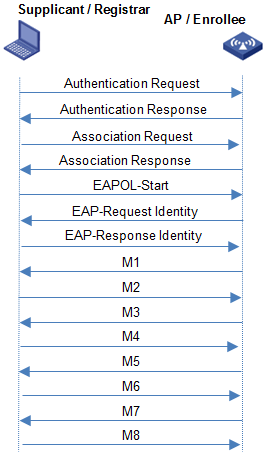
\includegraphics[width=0.3\textwidth]{./conversation}
  \end{center}
  \vspace{-20pt}
  \caption{WPS Pin Entry (External Registrar) verification diagram.}
  \vspace{-10pt}
\end{wrapfigure}
The diagram of Figure 1 shows a situation where certain client device (Supplicant) wants to connect to a network administered by a certain AP. Since both AP and client have the WPS Pin Entry (External Registrar) mechanism implemented, the client is prompted to enter the 8-digit PIN into a form as soon as he enters to the range of the AP. In the Figure we have skipped these first steps and we focus on the messages sent since the client enters the password until it gets full access to the network.

The first four messages (authentication and association process) are needed in order for the AP to recognize the supplicant; that way the AP will not drop further packets coming from that MAC address. Right after, three EAP messages are exchanged in order to initiate the WPS PIN process. This is needed because WPS is encapsulated in a expanded type of EAP. Once the EAP initiation is done, both supplicant and AP are renamed as Registrar and Enrollee, respectively, in order to follow the nomenclature given by the Wi-Fi Alliance. From now on, all packets (M1-M8) are encapsulated in EAP.

M1 and M2 contains Enrollee´s and Registrar´s Diffie-Hellman public key, respectively. M3 contains the PIN, encrypted and sent by the Enrollee. By doing this, the Registrar can verify (only if it also knows the PIN) that the Enrollee is legitimate. In M4, the first half of the PIN is sent from the Registrar to the Enrollee. M5 is then sent by the Enrollee as a acknowledgment of receipt of M4. In M6, the second half of the PIN is sent. M7 is then used as a acknowledgement of receipt of M6 and also for providing the Registrar with the information of the network (SSID and password, amongst others). M8 is used as a acknowledgment of receipt of M7. If the first or second half of the PIN sent by the Registrar were wrong, an EAP-NACK message would be sent from the Enrolle after M4 or M6, respectively. However, if the dialog finishes without any trouble, the Registrar is ready for sending/receiving messages to/from the network.

As Stefan Viehb\"{o}ck mentioned in \cite{stefan}, this procedure presents some weaknesses that makes WPS vulnerable to a brute-force attack. Due to the fact that the PIN is sent in two stages (M4 and M6), and because in case of failure the Enrollee answers with an EAP-NACK right after each of these stages individually, the PIN can be guessed separately in two groups of four digits instead of a single group of 8. This notably reduces the amount of PINs to be tried by an attacker in order to succeed. Specifically, from $10^8=100,000,000$ to $10^4+10^4=20,000$. Moreover, since the last digit of the PIN is used as a checksum (and it can be easily deduced from the rest of the digits), this amount decreases even more, from $10^4+10^4=20,000$ to $10^4+10^3=11,000$.

\paragraph{The attack}
A possible brute-force attack methodology (\cite{stefan,reaver}) could be as it follows,
\begin{enumerate}
\item Authenticate and associate to the target AP, then initiate EAP negotiation.
\item Send M4 (first half of the PIN). If Enrollee answers with an EAP-NACK instead of M5, increase one unit the first half of the PIN, deauthenticate yourself from the AP and go back to the first step. If not, send M6 (second part of the PIN).
\item If Enrollee answers to M6 with an EAP-NACK instead of M7, increase one unit the second half of the PIN, recalculate the checksum, deauthenticate yourself from the AP and go back to the first step. If not, save all data received in M7 and get ready to access to the network.
\end{enumerate}

\subsection{What safety measures can be carried out?}
\paragraph{PBC} Regarding the PBC vulnerability, MAC address filtering could be an option, however it would not completely solve the problem because the attacker could spoof the address from a legitimate client. There is yet no measure to properly protect this mechanism, the only way is by not using it. On the other hand, since this passive attack mainly implies an indefinite amount of time, it is considered as impractical.

\paragraph{PIN Entry} The only way of totally protecting a network from a WPS PIN brute-force attack is by disabling the WPS PIN Entry (External Registrar) mechanism in the AP (\cite{cisco,cert}). However, a less drastic solution can be found in order to make the brute-force attack impractical (\cite{stefan}): perform a lock-out in the AP every certain amount of attempts. As an example, if every 5 attempts the AP would lock-out for 60 minutes, the maximum attack time would be of almost 92 days. MAC address filtering is not a solution because of the same than in PBC.

\section{Conclusion}
In this essay we have presented the two main WPS mechanisms as well as their vulnerabilities. By doing this we have demonstrated that even though they facilitate the access to a very secure network (WPA/WPA2), they are a threat that can't be helped by any way but disabling them.


\begin{thebibliography}{N}
\bibitem{stefan} Stefan Viehb\"{o}ck, \textit{Brute forcing Wi-Fi Protected Setup}. Available at \url{http://sviehb.files.wordpress.com/2011/12/viehboeck_wps.pdf}, version 3.

\bibitem{alliance} Wi-Fi Alliance. \textit{How does Wi-Fi Protected Setup Work?}. Available at \url{http://www.wi-fi.org/knowledge-center/faq/how-does-wi-fi-protected-setup-work}, visited 01/11/2014.

\bibitem{reaver} Reaver-WPS. \textit{Brute force attack against Wifi Protected Setup}. Available at \url{https://code.google.com/p/reaver-wps/}, visited 01/11/2014.

\bibitem{wikipedia} Wikipedia. Wi-Fi Protected Setup. \url{http://en.wikipedia.org/wiki/Wi-Fi_Protected_Setup}, visited 01/11/2014.

\bibitem{cisco} Cisco Systems. \textit{Protecting Your Network from the Wi-Fi Protected Setup Security Hole}, \url{http://www.ciscopress.com/articles/article.asp?p=1847302}, last revised 12/03/2012

\bibitem{cert} Carnegie Mellon University. WiFi Protected Setup PIN brute force vulnerability, \url{http://www.kb.cert.org/vuls/id/723755}, last revised 10/05/2012.

\end{thebibliography}


\end{document}
